\label{sec:appA}
       
Figure~\ref{fig:appA:allxsec} shows the different cross-section contributing to the same-sign top quark pair production, as a function of the mediator mass. The elementary processes
involved in the cross-section calculation are shown in figure~\ref{fig:appA:feyn_prod_ss_all}.

\begin{figure}[!h!tpd]
  \centering    
  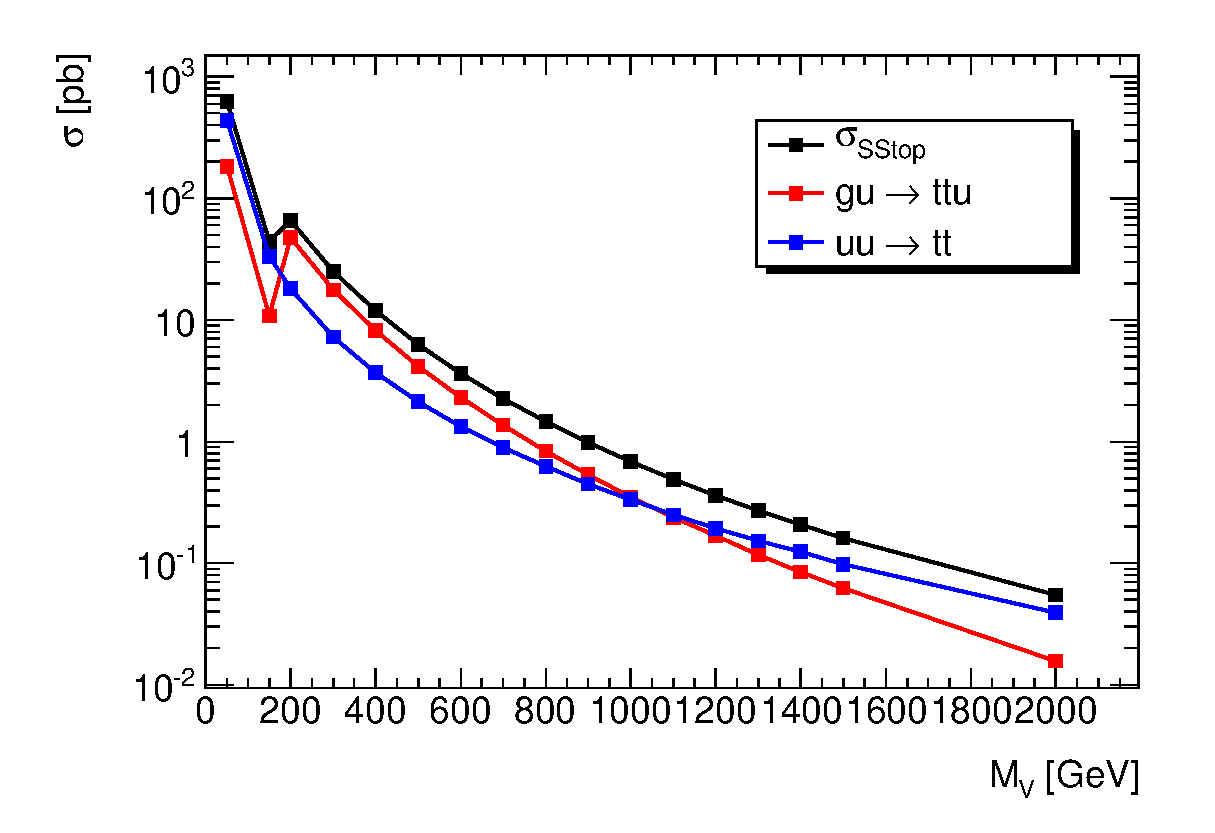
\includegraphics[width=0.6\textwidth]{appendix/appendixA/xsec_vs_mass.eps}
  \caption{
    Total cross-section of $tt\bar{u}$ (red) and $tt$ (bleue) production for different mediator mass. The total cross-section is shown in black.
  }
  \label{fig:appA:allxsec}
\end{figure}



Figure~\ref{fig:appA:fractionOftandvirtualV} shows how the various diagrams contribute to the total cross-section for the $tt+X$ final state, 
as a function of the mediator mass and for two different width. More precisely, there are two disctinct partonic 
processes: $gu \to tt\bar{u}$ ($\sigma(tt\bar{u})$) and $uu \to tt$ ($\sigma(tt)$). The total cross-section is written $\sigma(tt+X) \equiv \sigma(tt\bar{u}) + \sigma(tt)$.
The width which are considered in this section are the value calculated by MadGraph (labelled \textit{auto}) using the visible decay mode only, and a value set
by hand at $10\%$ of $m_V$.

\begin{figure}[!h!tpd]
  \centering
  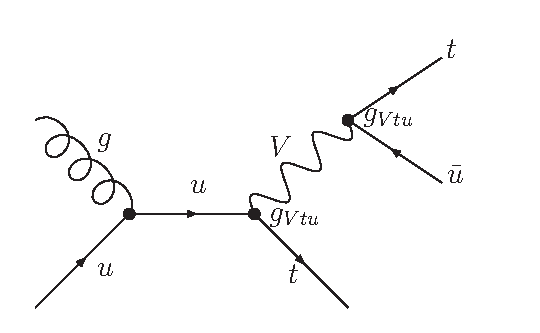
\includegraphics[width=0.23\textwidth]{feyn_diags/gu_Vt_tu}     \hspace{0.5cm}
  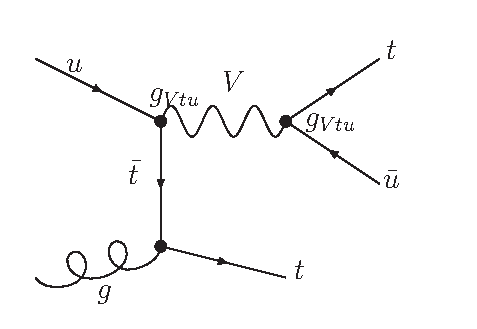
\includegraphics[width=0.23\textwidth]{feyn_diags/gu_Vt_tu_2}   \hspace{0.8cm}
  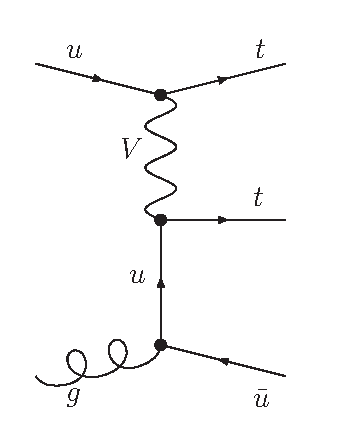
\includegraphics[width=0.13\textwidth]{feyn_diags/other_gu_ttu} \hspace{1.0cm}
  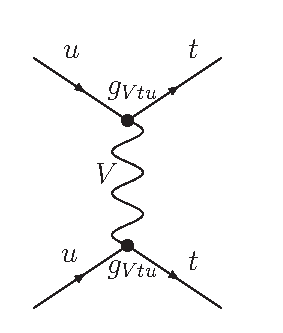
\includegraphics[width=0.13\textwidth]{feyn_diags/uu_tt}
  \caption{
    Feynman diagram of leading order processes leading to the $tt\bar{u}$ (left) and to the $tt$ production (right), both via $V$ exchange in the $t$-channel.
  }
  \label{fig:appA:feyn_prod_ss_all}
\end{figure}

The left plot of figure~\ref{fig:appA:fractionOftandvirtualV} shows the fraction $\sigma(tt) / \sigma(tt+X)$ as a function of
$m_V$. The observed behaviour is explained by the propagator of $V$: below the $m_t$ threshold, $V$ can only be virtual and the $t$-channel has a large contribution.
At high mass, it becomes more and more difficult to produce an on-shell $V$ which makes the $t$-channel fraction larger as the mass increases. This is even
more pronounced when $\Gamma_V$ increases since it makes the probability to be virtual higher.

The right plot of figure~\ref{fig:appA:fractionOftandvirtualV} shows the impact of third diagram from figure~\ref{fig:appA:feyn_prod_ss_all} on the $tt\bar{u}$ production. 
Indeed, $V$ doesn't decay into $t\bar{u}$ in this diagram, in opposition to the diagrams describing $gu \to tV(\to t\bar{u})$. Practically, 
the fraction of $gu \to tt\bar{u}$ events with an on-shell $V$\footnote{This is defined by a Madgraph parameter $bwcut$, 
standing for Breit-Wigner Window. If $\sqrt{E_V^2 - {\vec{p}_V}^2}$ is in a window of $bwcut \times \Gamma_V$ centered to $m_V$, then $V$ is considered as on-shell. For this study, $bwcut=25$.} compared 
to all $gu \to tt\bar{u}$ events. More the $V$ width is large, more this effect is visible. The interest of this plot is to quantify the fraction of events 
which cannot be simply scaled by $\BR{V}{\chi\chi}$ for the monotop and same-sign combination (cf.~\ref{sec:comb}).

\begin{figure}[!h!tpd]
  \centering
  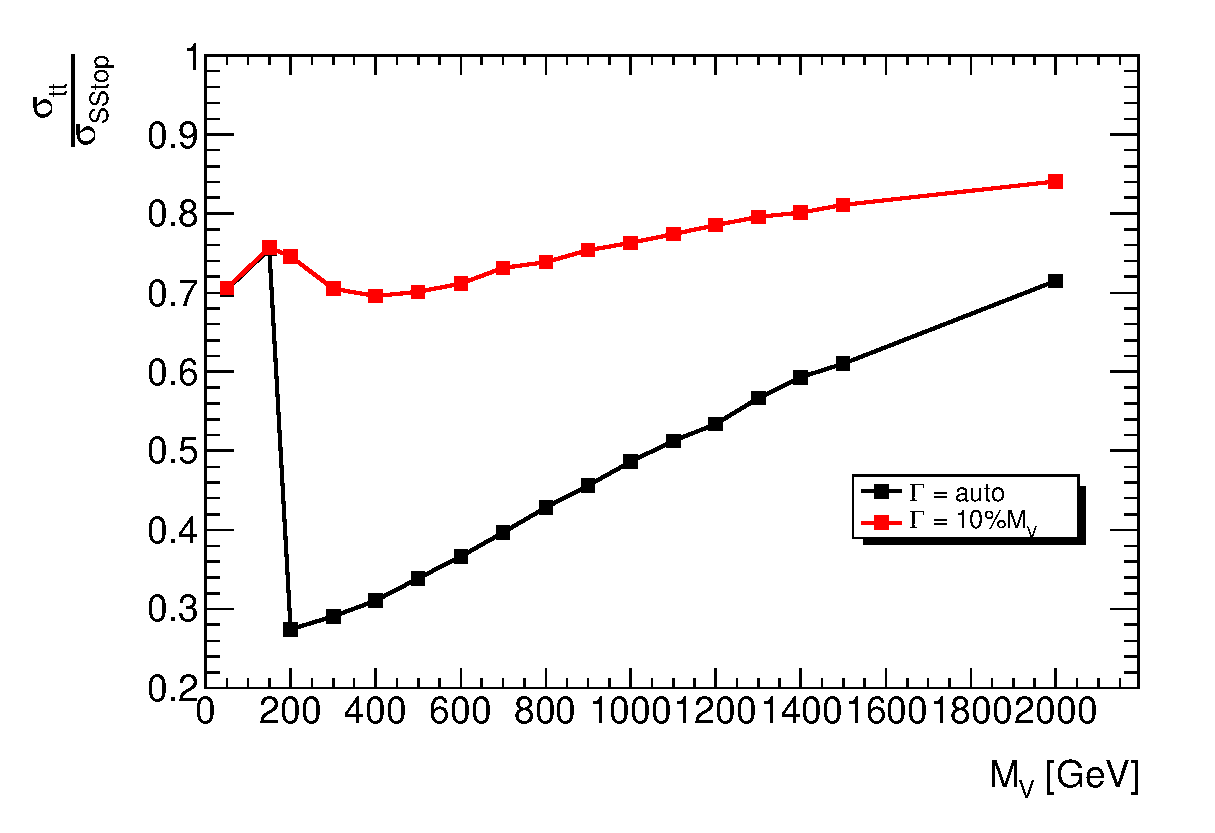
\includegraphics[width=0.48\textwidth]{appendix/appendixA/uu_tt_ratio_vs_mass.eps}
  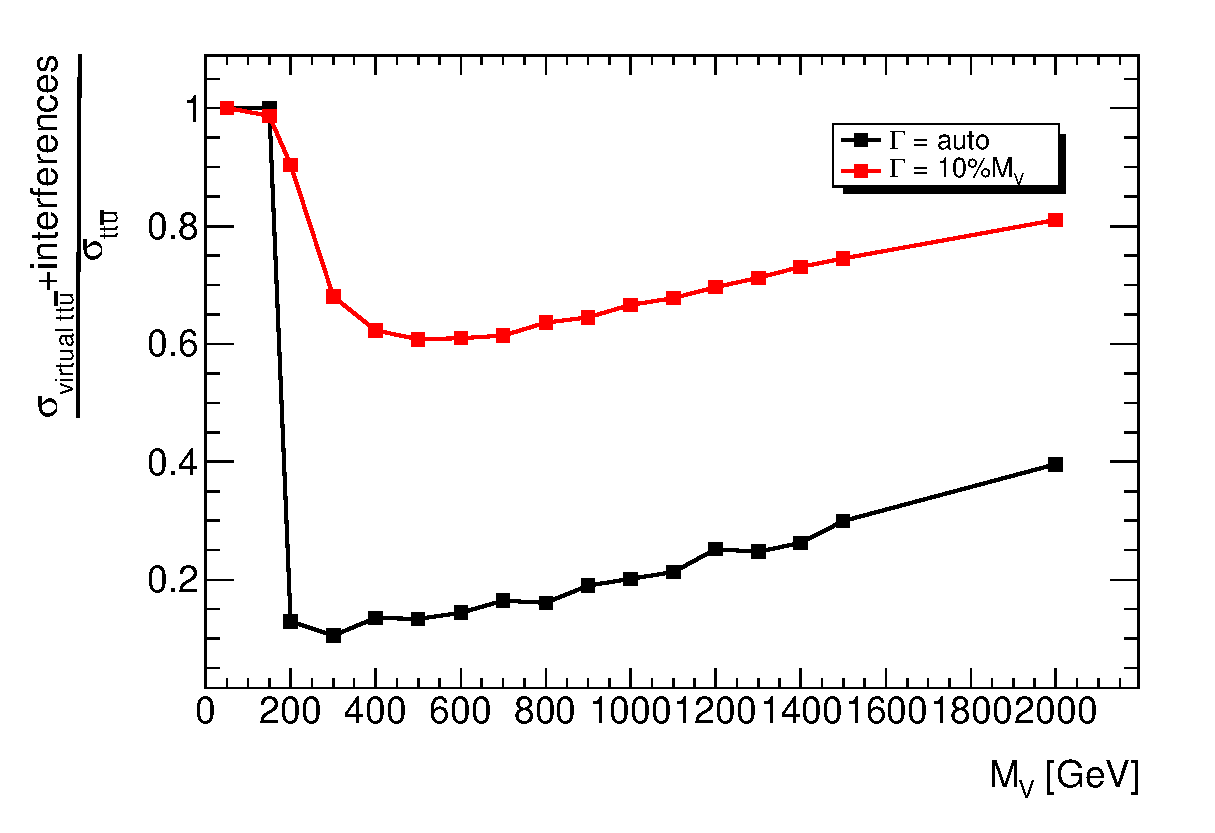
\includegraphics[width=0.48\textwidth]{appendix/appendixA/virtual_ttu_ratio_vs_mass.eps}
  \caption{
    Fraction of $t$-channel for the $tt+X$ final state as a function of the mediator mass (left) and effect of virtual $V$ contribution to 
    $gu \to tt\bar{u}$ process as a function of the mediator mass (right).
  }
  \label{fig:appA:fractionOftandvirtualV}
\end{figure}
